	Following \citeA{stock1988probability, stock&watson1989indexes}, we take data on Industrial Production (IP), total personal income less transfer payments (GMYXP), total manufacturing and trade sales (MT82), and employee-hours in non-agricultural establishments (LPMHU). Note that in their first paper \citeyear{stock1988probability} they use employes on non agricultural payrols.  The reason of this change is to following Moore's (1988) recommendation. Because of over time and part-timework, employee-hours measures more directly fluctuations in labour input than does the number of employees. Hence, our results are goning to be different from those of \citeA{stock1988probability} for that reason. Data has been downloaded from Stock's \href{https://www.princeton.edu/~mwatson/publi.html}{webpage}.  %Note that my data is different from those used by \citeA{stock&watson1989indexes}. I am taking data from 2014-12-15 to 2022-08-31.
\begin{figure}[h!]
	\centering
	\captionsetup{width=0.5\textwidth, font=small}
	\caption{$C_{t|t}$ together with a 5\% confidence interval (assuming gaussianity).}\label{fig:cei}
	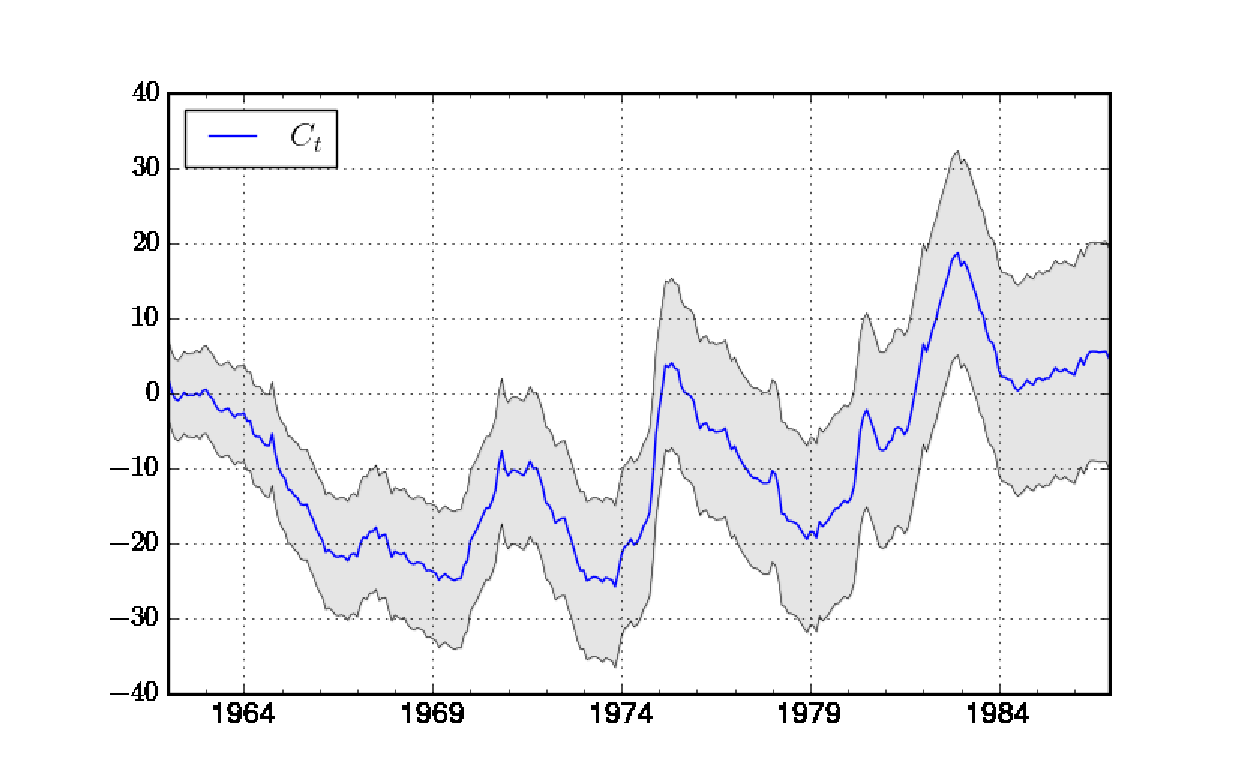
\includegraphics[scale=0.5]{fig/sw_CEI}
\end{figure}
% employees on non agricultural payrolls.
	\subsection{Preliminary analysis}
	
	The first step in specifying the model is to test for whether the series are integrated and, if they are, whether they are cointegrated.  As in \citeA{stock1988probability, stock&watson1989indexes}, for each of the the coincident indicators, \citeA{dickey1979distribution} test for a unit root (against the alternative that the series are stationary, perhaps around a linear time trend) was unable to reject (at the 10\% level) the hypothesis that the series are integrated. P-values are reported in Table \ref{tab:df_pvalues}.
	
	\begin{table}[h!]
		\centering\small
		\captionsetup{width=0.6\textwidth, font=small}
		\caption{P-values of the test \protect\citeA{dickey1979distribution} for a unit root applied to the four series used in the index estimation. We fail to reject in every case at thte 10\%.}\label{tab:df_pvalues}
		\vspace{0cm}
		\begin{tabular}{l|rrrr}

{} &    IP & GMYXP8 &  MT82 & LPMHU \\ \hline\hline

p value &  0.97 &   0.99 &  0.98 &  0.99 \\ \hline\hline

\end{tabular}

	\end{table}
 
	The subsequent aplication of the \citeA{engle1987co} test of the nul hypothesis that the four series are not cointegrated against the alternative of cointegration failed to reject at the 10\% significance level. Thus these tests provided no evidence against the hypothesis that each series is integrated but they are not cointegrated. I therefore estimated the model using for the first diference of the logarithm of each of the coincident series, standardized to have zero mean and unit variance.

	\begin{table}[h!]
		\centering\small
		\captionsetup{width=0.6\textwidth, font=small}
		\caption{P-values of the \protect\cite{engle1987co} for cointegration to the four series used in the index estimation. We fail to reject in every case at the 10\% level.}
		\begin{tabular}{l|rrrr}

{} &        IP &    GMYXP8 &      MT82 &     LPMHU \\ \hline\hline

IP     &       - &  0.013209 &  0.230167 &  0.000807 \\
GMYXP8 &   0.01397 &       - &  0.020279 &  0.128943 \\
MT82   &  0.248144 &  0.020003 &       - &  0.121991 \\
LPMHU  &  0.051041 &  0.134312 &  0.130508 &       - \\ \hline\hline

\end{tabular}

	\end{table}

\subsection{Maximum Likelihood Estimation}

The parameters of the single-index model have been estimated using IP, DPI, TS and AW over the periods 1959:2-1983:12. As in \citeA{stock&watson1989indexes}, a second order autoregressive  specification  has been adopted for $\Delta C_t$, so that $p=2$. Also, errors $u_t$ are modelled as an $AR(2)$, i.e., $k=2$. I have followed \citeA{stock1988probability} and considered $\gamma$ to be constant, i.e., $\gamma = \gamma_0\in\R^4$. The loglikelihood for this model is 424.529. The maximum likelihood estimates of the parameters of the single-index model are presented in Tables  he maximum likelihood estimates of the parameters of the single-index model are presented in Table \ref{tab:sw-ml-params}. I have follow \citeA{gupta1974computational} for maximising the log likelihood.The basic idea is that the negative log likelihood is minimised by the Newton-Raphson Method, iterating the process until the log likelihood stabilises. Standard errors are computed as the square root of the diagonal of the (approximated) Hessian matrix of $\mathcal{L}$.

\begin{table}[h!]
\centering\captionsetup{width=0.8\textwidth, font=small}
\caption{The estimation period is 1959:2-1983:12. The parameters were estimated by Gaussian maximum likelihod as described in the text. The parameters are $\gamma = (\gamma_1,\ldots, \gamma_4)$, $D(L)=\text{diag}\left(d_1(L),\ldots, d_4(L)\right)$, where $d_i(L) = 1-d_{i1}L - d_{12}L^2$ and $\Sigma = \text{diag} \left(1,\sigma_1^2,\ldots,\sigma_4^2\right)$. Maximum likelihood is $\mathcal{L}=424.529$.}\label{tab:sw_ml-params}
\begin{tabular}{l|cccc}
&IP&GMYX&LPMH&LPMHU\\\hline\hline
$\gamma_i$&-0.7219&-0.4976&-0.4625&-0.5001\\
&(0.033)&(0.0283)&(0.0283)&(0.0274)\\
$d_{1i}$&-0.0204&-0.1163&-0.4273&-0.4453\\
&(0.0858)&(0.1191)&(0.0769)&(0.0489)\\
$d_{2i}$&-0.1492&0.1513&-0.2311&-0.1206\\
&(0.1071)&(0.0515)&(0.0996)&(0.0675)\\
$\sigma_i$&0.4681&0.78&0.7425&0.7132\\&(0.0362)&(0.033)&(0.0309)&(0.0308)\\\hline\hline
\end{tabular}
\end{table}
The CEI, $C_{t|t}$,  is is plotted in Figure \ref{fig:cei}. Notice that  $$C_{t|t} = [Z_c \ 0 \ 1] \hat{\alpha}_{t|t}.$$ I have also included a 5\% confidence interval band measured by $$C_{t|t}\pm 1.96 \sqrt{\hat{P}_{t|t}},$$ where $$\hat{P}_{t|t} = [Z_c \ 0 \ 1] \hat{\alpha}_{t|t}[Z_c \ 0 \ 1]^{\text{\tiny T}}$$


%	\begin{table}[h!]
%		\centering\small
%			\captionsetup{width=0.6\textwidth, font=small}
%			\caption{The estimation period is 2006:12-2022:08. The parameters were estimated by Gaussian maximum likelihod as described in the text. The parameters are $\gamma = (\gamma_1,\ldots, \gamma_4)$, $D(L)=\text{diag}\left(d_1(L),\ldots, d_4(L)\right)$, where $d_i(L) = 1-d_{i1}L - d_{12}L^2$ and $\Sigma = \text{diag}\left(1,\sigma_1^2,\ldots,\sigma_4^2\right)$. Maximum likelihood is $\mathcal{L}=274.819$ at the 42688th iteration.}\label{tab:ml-params1}
%		\begin{tabular}{l|rrrr}
%			& IP & DPI & TS & AW \\\hline\hline
%			$\gamma_i$ & 0.592400 & -0.160700 & 0.585400 & 0.320700 \\
%			$d_{1i}$ & -0.136700 & -0.277700 & 0.298100 & -0.857200 \\
%			$d_{2i}$ & -0.010300 & -0.796800 & -0.288700 & -0.060500 \\
%			$\sigma_{i}$ & 0.399400 & 0.611400 & 0.013000 & 0.831200 \\\hline\hline
%			&\multicolumn{2}{c}{$\phi_1$} & \multicolumn{2}{c}{$\phi_1$}  \\\hline\hline
%			&\multicolumn{2}{c}{0.994600} & \multicolumn{2}{c}{0.639000} \\\hline
%		\end{tabular}
%	\end{table}

%	
%
%	\begin{figure}[h!]
%		\centering
%		\captionsetup{width=0.6\textwidth, font=small}
%		\caption{Evolution of the maximum likelihood, $\mathcal{L}$, during the iteration process. X-axis is plotted in log-scale.}
%		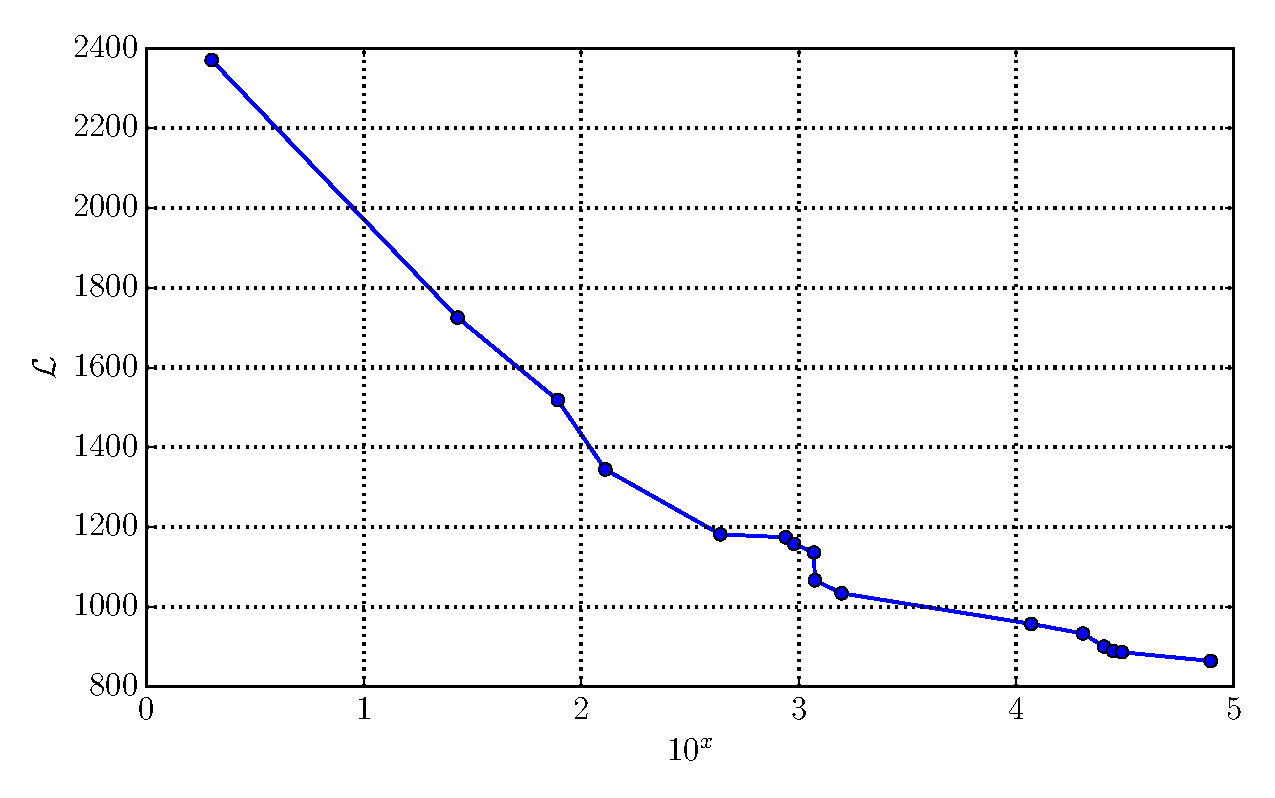
\includegraphics[scale=0.5]{fig/L.eps}
%	\end{figure}
%
%		\begin{figure}[h!]
%		\centering
%		\setlength{\abovecaptionskip}{1pt}
%		\captionsetup{width=0.6\textwidth, font=small}
%		\caption{$C_{t|t} = \begin{bmatrix}
%				Z_c & 0 & 1
%			\end{bmatrix} \alpha_{t|t}$.}
%		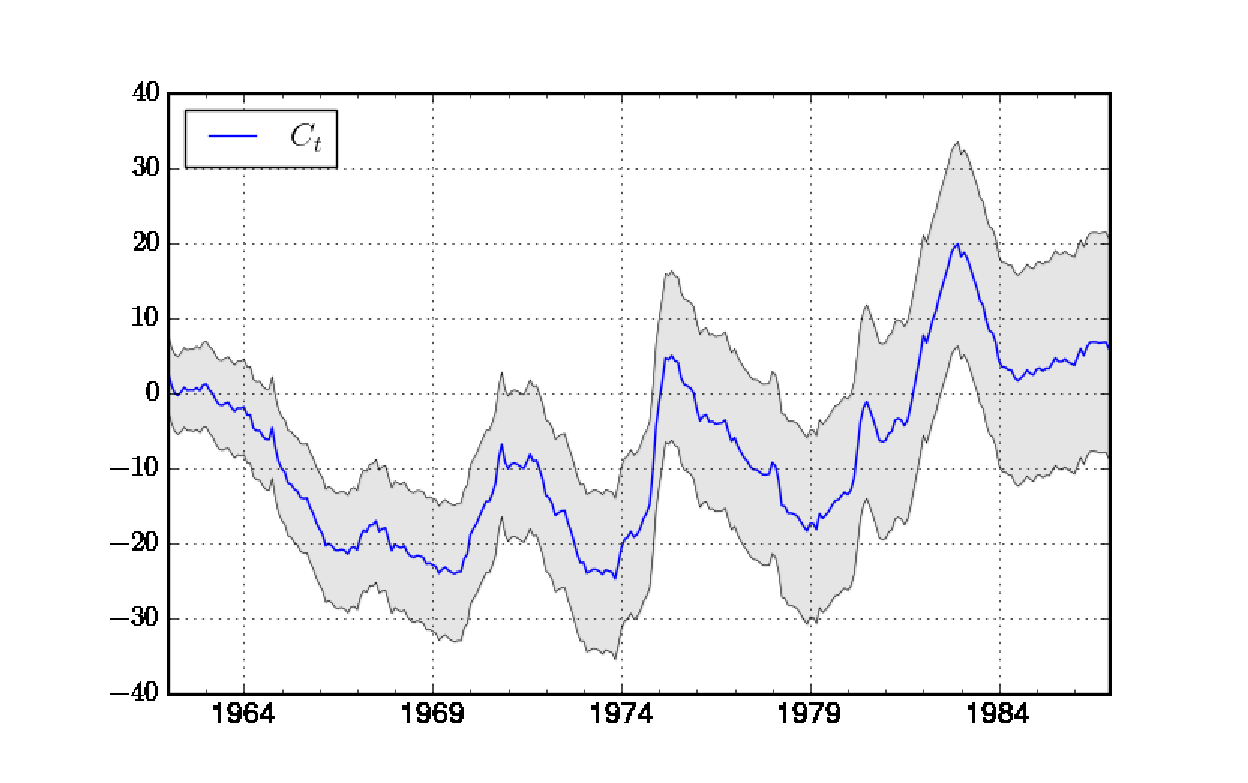
\includegraphics[scale=0.6]{fig/CEI.eps}
%	\end{figure}
% IP: aUSIPMANG/CA
% DPI: aUSGPYDPC/CA
% TS: aUSWSLS/A
% AW: USWRKW=ECI
